% !TEX root = main.tex

\section{Experiments}
\label{sec:exp}

In this section, we present our experimental study.
We use DBpedia~\cite{dbpedia} and Probase~\cite{wu2012probase} as our knowledge repository.
\nop{We use entity pair as well as their attributes in DBpedia to learn the conceptual patterns.
We use Probase for conceptualization. We carry out all the experiments on a PC with Intel i7 cpu @2.5Ghz and 16G memory. All the programs are implemented in Python.
}
\
\vspace{-4mm}
\paragraph*{Evaluation Metrics}
%Given a pair of entities, our system produces the most plausible top-K attributes between them.
We need to evaluate how accurate the result is. 
Hence, we use $nDCG@K$ and $MAP@K$ as our evaluation metric.
We further use $ ERR@K$ ( {\it Expected Reciprocal Rank})~\cite{chapelle2009expected} to evaluate the our collective conceptualization procedure.
For all the metrics, a larger values always imply a better result. We ask volunteers to label the goodness of all results.
%, evaluating the correctness of first $K$ concept pairs is similar to user browsing case. In our case, a user may stop looking at more concepts if top-$K$ concepts already provide sufficient conceptual information for the entity pair.
% 我突然想到了我这里做过个优化, 每次算concept pairs 的时候按照P(C|E)排个序,如果排在后面的c,乘上最大的P(<c1,c2>|a)P(a)也不能超过前面的,就停止搜索了。2015年9月15日19:23:27

\vspace{-4mm}
\paragraph*{Exp 1: Effectiveness of $ERF$}
In this experiment, we evaluate the effectiveness of our $ERF$ system.
We first show that $ERF$ systems can explain relationship for most entity pairs.
We compare to a baseline that directly retrieves the attribute from DBpedia for the entity pair.
We randomly select 50 Wikipedia article (entity $e_1$) and the hyper-linked entities in its abstract (entity $e_2$)
to construct query entity pairs.
%The result is reported in Table~\ref{tab:precision_compare}.
Overall, $ERF$ can generate correct attributes for 83\% entity pairs.
Our system explains 15.77\% more entity pairs than the baseline (64\%).

%\nop{
%Since we assume 0 if the entity has no relation can be retrieved from database and otherwise 1, the average $Precision@1$ results here can also be viewed as \ac{recall} of the knowledge base.
%DBpedia provides only one relation for a covered entity pair, therefore we use $Precision@1$ to compare the results.
%Our $ERF$ method improves the average $Precision@1$ by 15.77\%.
%}

%\nop{
%\begin{table}[htbp]
%  \centering
%  \caption{Precision@1 Compared With Baseline}
%    \begin{tabular}{rrr}
%    \toprule
%         & P@1  & \%Improv. \\
%    \midrule
%    Dbpedia direct & 0.64 & -- \\
%    $ERF$  & 0.83 & 15.77 \\
%    \bottomrule
%    \end{tabular}%
%  \label{tab:precision_compare}%
%\end{table}%
%}


To further justify the effectiveness of $ERF$, we compare two versions of our solution, one with head-aware conceptualization ($ERF-H$)
and one with direct conceptualization ($ERF-D$).
We report all the precision metrics in Table~\ref{tab:ndcg}. 
The results show that both of two versions of $ERF$ can consistently achieve accuracy above 0.87 on different metrics.
$ERF-H$ performs best. In most metrics, it has an accuracy larger than 0.9. In the next experiments, without extra statement, we
always report the result of $ERF-H$.


\begin{table}[!htbp]
\vspace{-4mm}
\small	
  \centering
  \caption{Evaluation Result}
	% Table generated by Excel2LaTeX from sheet 'Sheet1'
% Table generated by Excel2LaTeX from sheet 'Sheet1'
	\begin{tabular}{lrrrr}
	\toprule
	     & nDCG@3 & nDCG@5 & MAP@3 & MAP@5 \\
	\midrule
	$ERF-D$ & 0.925 & 0.887 & 0.916 & 0.87 \\
	$ERF-H$ & 0.928 & 0.933 & 0.902 & 0.907 \\
	\bottomrule
	\end{tabular}%

  \label{tab:ndcg}%
%  \vspace{-4mm}
\end{table}%



\vspace{-4mm}
\paragraph*{Exp 2: Head-aware Conceptualization}
In this experiment, we show that head-aware conceptualization significantly reduces the computational cost without sacrificing precision. 
In Table~\ref{tab:nhc}, we report the statistics of Probase concept space and head concepts with isA concurrence number rectified by its long concepts. 
We can see that the number of head concepts is only 1.5\% of Probase concept number. This brings a significant reduction in computation. 
The increase of \emph{average \#occurrence} indicates the confidence of the $e$ \isa $c$ pair is increased.
%The increase of the average children per concept makes entities less unique, which will help avoid entity with same head concept share no long concept.


\begin{table}[htbp]
\vspace{-4mm}
  \centering
  \caption{Statistics of Head-aware Conceptualization}
  \small
    \begin{tabular}{rrrr}
    \toprule
          & Before & After & Changed\% \\
    \midrule
    \#concept & 2127953 & 33197 & -98.44 \\
    average \#occurrence & 1.75  & 2.71  & 54.85714 \\
   % \#children per concept & 7.53  & 184.3 & 2347.543 \\
  %  \#parents per entity & 2.33  & 1.55  & -33.4764 \\
    \bottomrule
    \end{tabular}%
  \label{tab:nhc}%
\end{table}%


We give the distribution of head concepts without ($P(h|e)$) and with rectification ($\hat{P^*}(h|e)$).  Figure~\ref{fig:hac} illustrate the distribution, from which we can observe that (1) $P(h|e)$ and $\hat{P^*}(h|e)$ in general is positively correlated to each other with a Pearson correlation coefficient as {\bf 0.89} (2) for important heads (with large $P(h|e)$) their conditional probability is amplified. These results suggest that we derived an estimation in a smaller concept space without losing the accuracy.


\begin{figure}[!tb]
%\vspace{-8mm}
\centering
\small
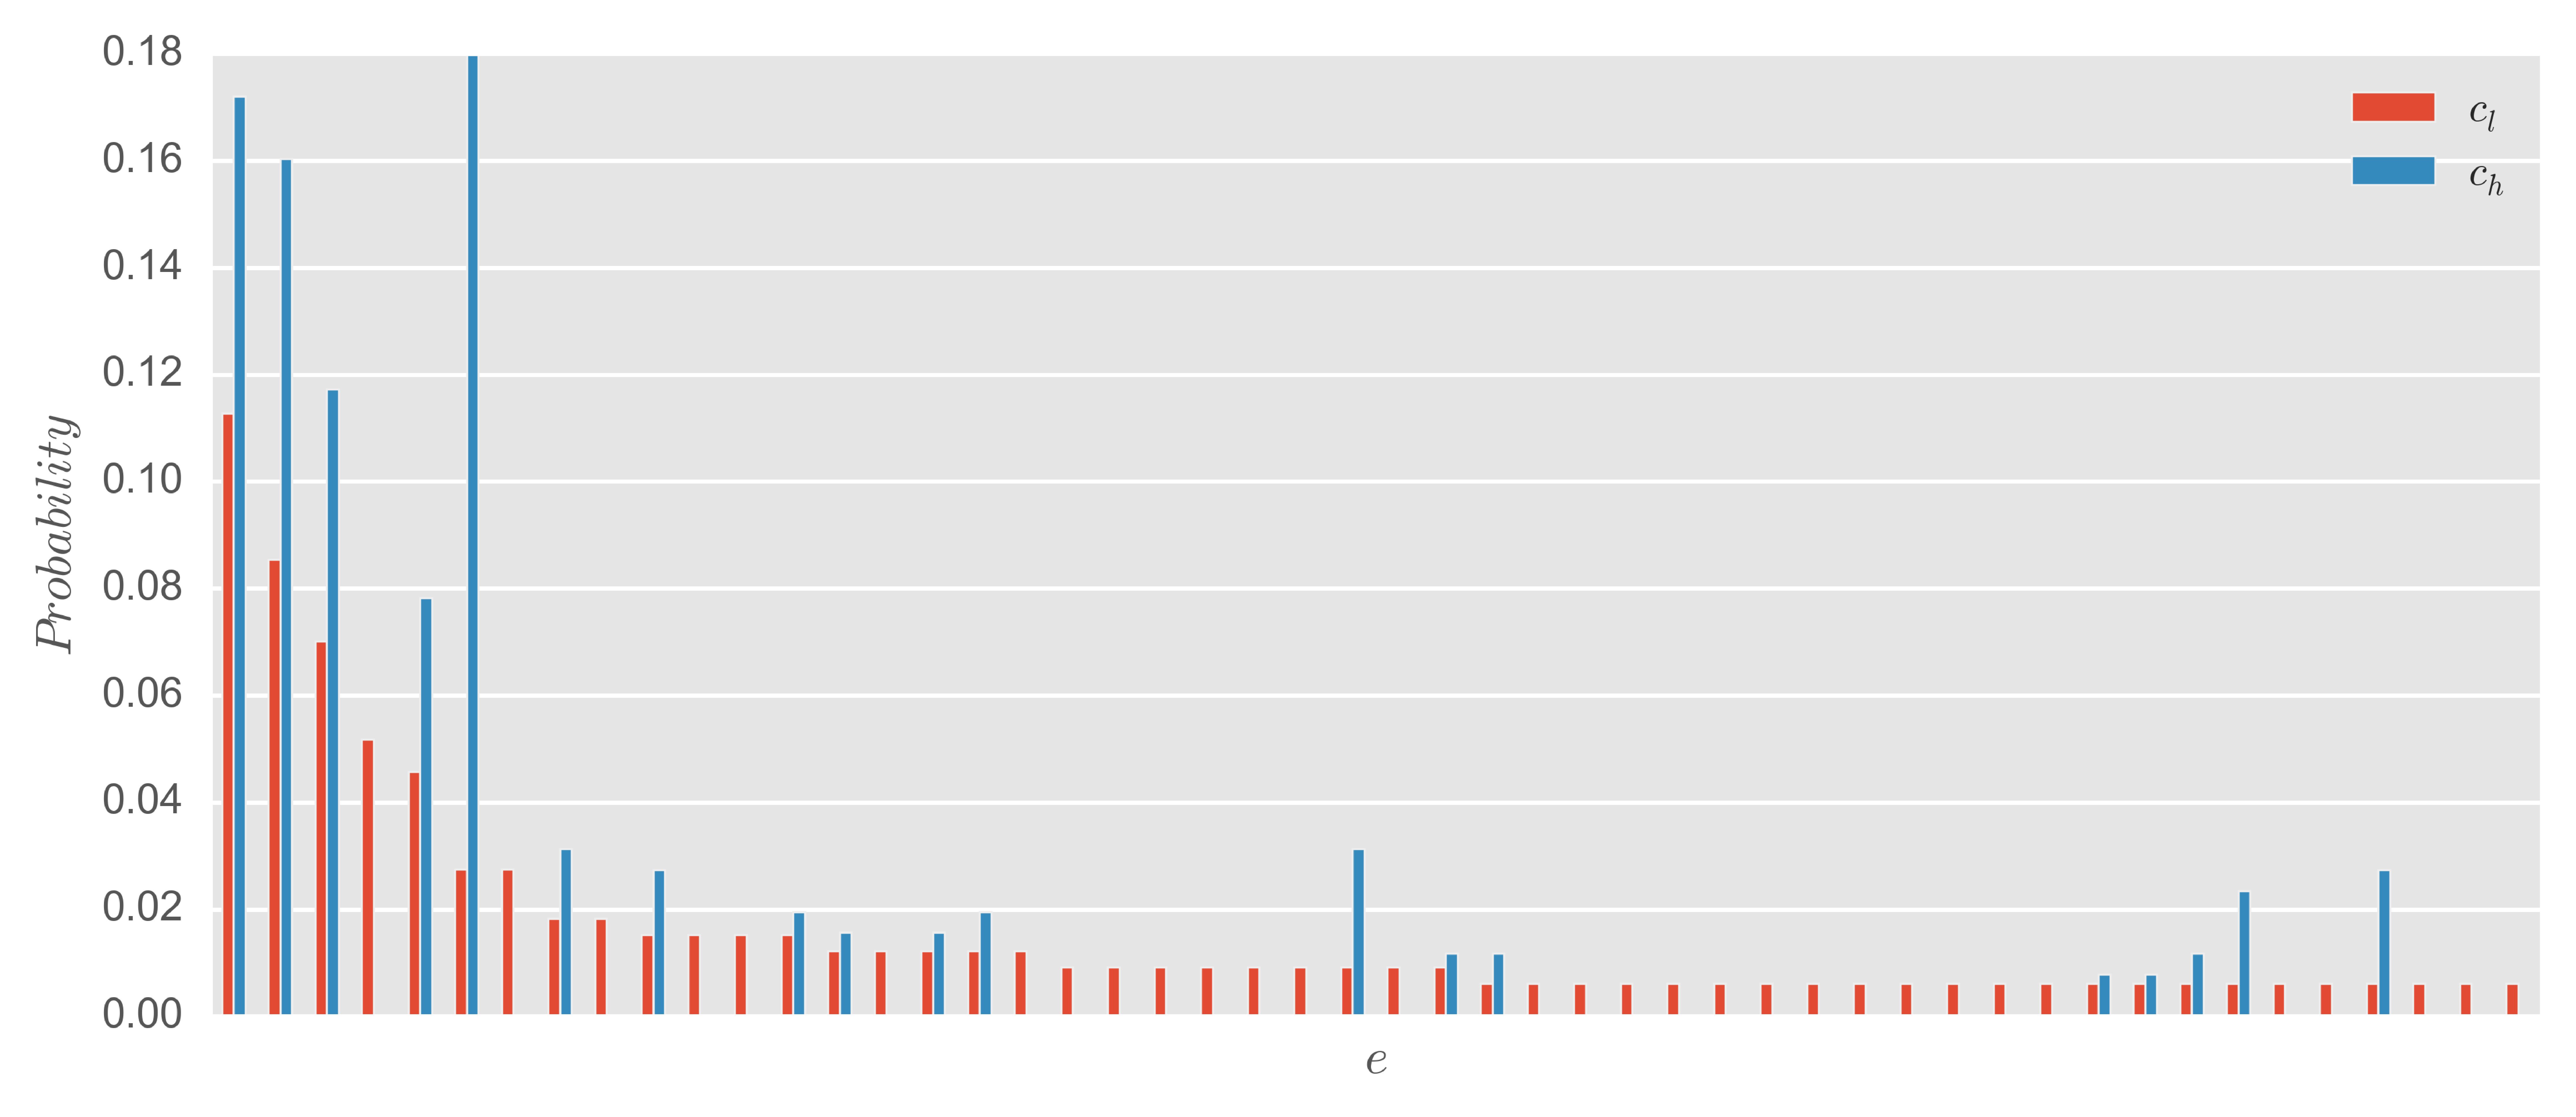
\epsfig{file=resources/df_hac_50_bill_gates.eps,width=\columnwidth, height=0.3\columnwidth}
\vspace{-8mm}
\caption{Comparison between $P(h|e)$ and $\hat{P^*}(h|e)$ for \at{Bill Gates}. \small The red bars means $P(h|e)$ and the blue ones represents $\hat{P^*}(h|e)$. }
\label{fig:hac}
\vspace{-6mm}
%
\vspace{-6mm}
\end{figure}


%
%\begin{table*}[htbp!]
%  \centering
%  \caption{Rerank comparation}
%    \begin{tabular}{llrrlrr}
%    \toprule
%    \multicolumn{1}{c}{} & \multicolumn{3}{c}{aggregated} & \multicolumn{3}{c}{original head concepts} \\
%    \midrule
%    \multicolumn{1}{c}{Entity} & agg head & agg count & agg prob & org head & org count & org prob \\
%    \midrule
%    \multicolumn{1}{c}{\multirow{10}[0]{*}{shanghai}} & city  & 1311  & 0.829222 & city  & 644   & 0.407337 \\
%    \multicolumn{1}{c}{} & region & 46    & 0.029096 & region & 27    & 0.017078 \\
%    \multicolumn{1}{c}{} & area  & 42    & 0.026565 & metropolis & 23    & 0.014548 \\
%    \multicolumn{1}{c}{} & metropolis & 26    & 0.016445 & megacities & 15    & 0.009488 \\
%    \multicolumn{1}{c}{} & port  & 20    & 0.01265 & market & 15    & 0.009488 \\
%    \multicolumn{1}{c}{} & market & 19    & 0.012018 & location & 15    & 0.009488 \\
%    \multicolumn{1}{c}{} & centre & 18    & 0.011385 & port  & 9     & 0.005693 \\
%    \multicolumn{1}{c}{} & location & 17    & 0.010753 & locality & 6     & 0.003795 \\
%    \multicolumn{1}{c}{} & megacities & 15    & 0.009488 & locale & 5     & 0.003163 \\
%    \multicolumn{1}{c}{} & center & 11    & 0.006958 & seaport & 4     & 0.00253 \\
%          &       &       &       &       &       &  \\
%    \multicolumn{1}{c}{\multirow{10}[0]{*}{bill gates}} & leader & 46    & 0.140244 & billionaire & 37    & 0.112805 \\
%    \multicolumn{1}{c}{} & billionaire & 44    & 0.134146 & entrepreneur & 28    & 0.085366 \\
%    \multicolumn{1}{c}{} & entrepreneur & 41    & 0.125 & philanthropist & 23    & 0.070122 \\
%    \multicolumn{1}{c}{} & philanthropist & 30    & 0.091463 & celebrity & 15    & 0.045732 \\
%    \multicolumn{1}{c}{} & celebrity & 20    & 0.060976 & leader & 9     & 0.027439 \\
%    \multicolumn{1}{c}{} & person & 16    & 0.04878 & innovator & 6     & 0.018293 \\
%    \multicolumn{1}{c}{} & figure & 11    & 0.033537 & personality & 5     & 0.015244 \\
%    \multicolumn{1}{c}{} & innovator & 8     & 0.02439 & expert & 5     & 0.015244 \\
%    \multicolumn{1}{c}{} & luminary & 8     & 0.02439 & folks & 4     & 0.012195 \\
%    \multicolumn{1}{c}{} & individual & 7     & 0.021341 & icon  & 4     & 0.012195 \\
%          &       &       &       &       &       &  \\
%    \multicolumn{1}{c}{\multirow{10}[0]{*}{samsung}} & company & 1030  & 0.376875 & company & 816   & 0.298573 \\
%    \multicolumn{1}{c}{} & brand & 829   & 0.30333 & brand & 561   & 0.205269 \\
%    \multicolumn{1}{c}{} & manufacturer & 238   & 0.087084 & client & 42    & 0.015368 \\
%    \multicolumn{1}{c}{} & maker & 112   & 0.040981 & firm  & 39    & 0.01427 \\
%    \multicolumn{1}{c}{} & player & 60    & 0.021954 & rival & 38    & 0.013904 \\
%    \multicolumn{1}{c}{} & phone & 60    & 0.021954 & player & 33    & 0.012075 \\
%    \multicolumn{1}{c}{} & giant & 51    & 0.018661 & phone & 30    & 0.010977 \\
%    \multicolumn{1}{c}{} & firm  & 49    & 0.017929 & conglomerate & 19    & 0.006952 \\
%    \multicolumn{1}{c}{} & name  & 49    & 0.017929 & corporation & 19    & 0.006952 \\
%    \multicolumn{1}{c}{} & conglomerate & 42    & 0.015368 & partner & 12    & 0.004391 \\
%          &       &       &       &       &       &  \\
%    \multicolumn{1}{c}{\multirow{10}[0]{*}{mona lisa}} & painting & 56    & 0.4   & painting & 33    & 0.235714 \\
%    \multicolumn{1}{c}{} & masterpiece & 21    & 0.15  & masterpiece & 16    & 0.114286 \\
%    \multicolumn{1}{c}{} & work  & 20    & 0.142857 & work  & 10    & 0.071429 \\
%    \multicolumn{1}{c}{} & film  & 6     & 0.042857 & film  & 5     & 0.035714 \\
%    \multicolumn{1}{c}{} & image & 5     & 0.035714 & image & 3     & 0.021429 \\
%    \multicolumn{1}{c}{} & artwork & 4     & 0.028571 & picture & 3     & 0.021429 \\
%    \multicolumn{1}{c}{} & portrait & 4     & 0.028571 & treasure & 2     & 0.014286 \\
%    \multicolumn{1}{c}{} & piece & 4     & 0.028571 & song  & 2     & 0.014286 \\
%    \multicolumn{1}{c}{} & picture & 3     & 0.021429 & icon  & 2     & 0.014286 \\
%    \multicolumn{1}{c}{} & figure & 3     & 0.021429 & artwork & 1     & 0.007143 \\
%    \bottomrule
%
%    \end{tabular}%
%  \label{tab:rerank}%
%\end{table*}%



%\subsection{Find alias}

%\subsubsection{compare}
%
%In this section we compare $ P(<c_1,c_2 >|a )$ with $ P(c_1|a) \times P(c_2|a)$ to show that

\begin{figure*}[htb]
\vspace{-12mm}
\centering
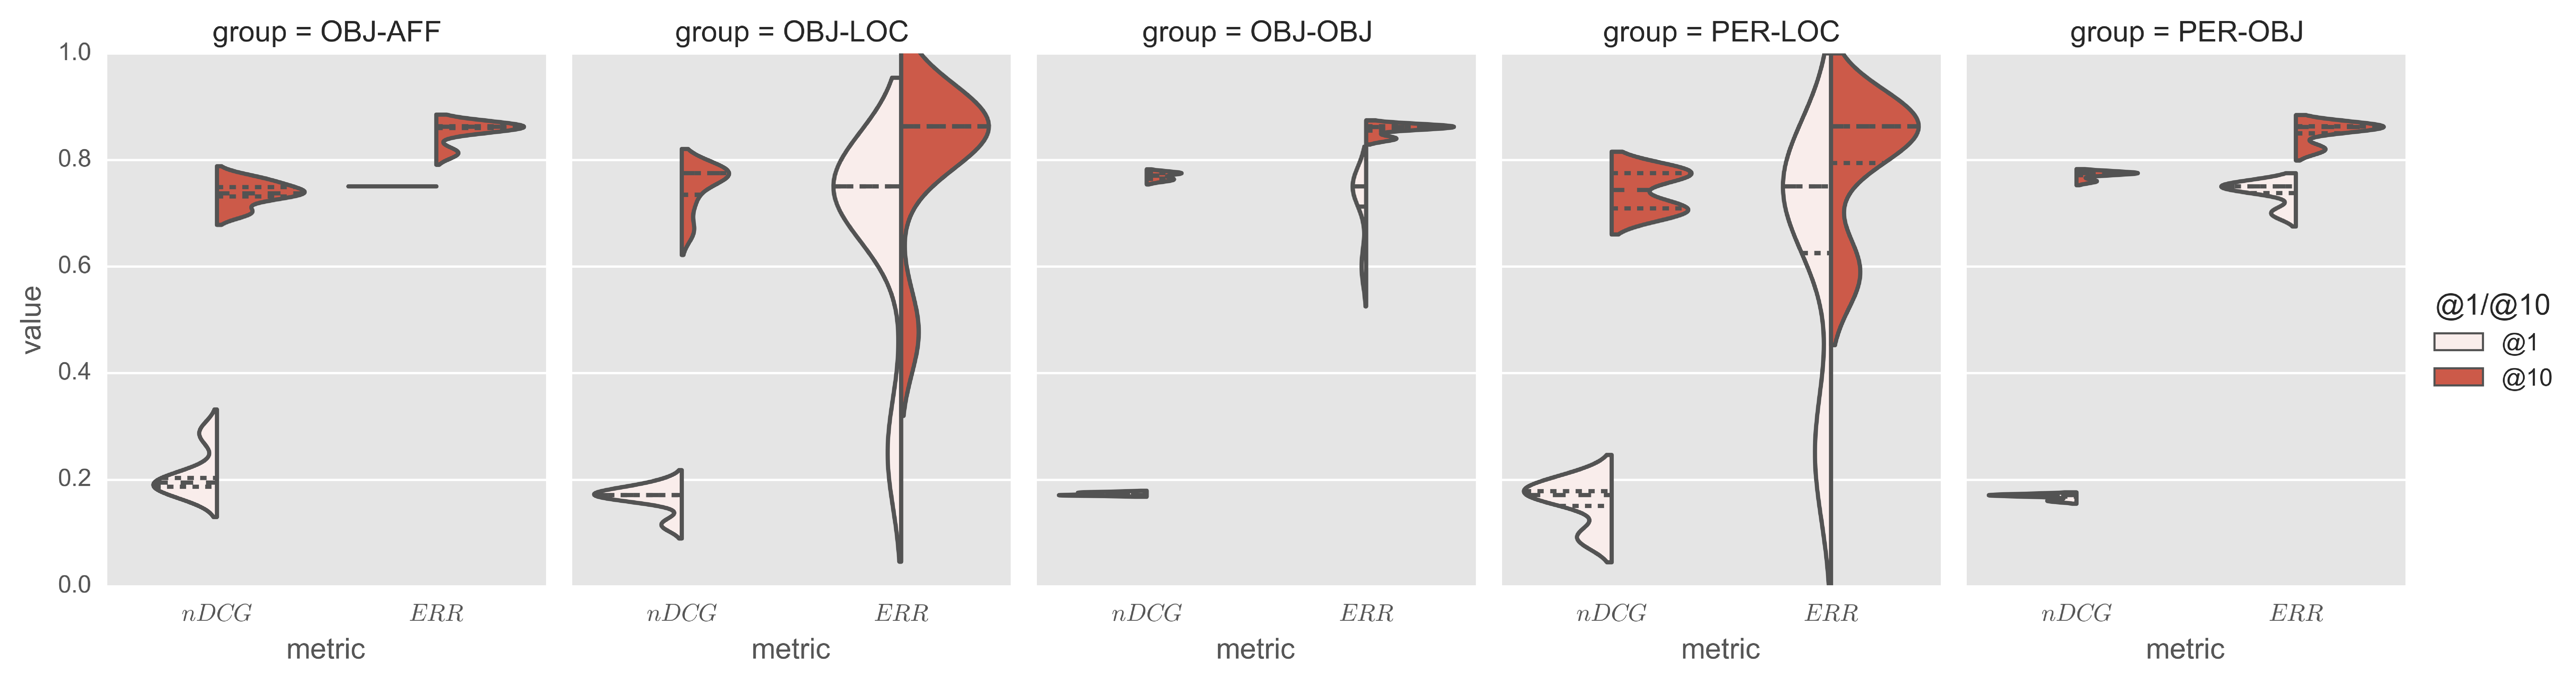
\epsfig{file=resources/violin_eval_group.eps,width=2.2\columnwidth}
\vspace{-8mm}
\caption{Distribution of human evaluation result for $P(\langle c_1,c_2 \rangle|a)$ produced by $ERF$. \small Each seperate graph represents a certain relation group.}
\label{fig:eva_violin_group}
\vspace{-10mm}
\end{figure*}

\vspace{-4mm}
\paragraph*{Exp 3: Joint Conceptualization}
Now, we evaluate the effectiveness of joint conceptualization, which is implemented by the introduction of $\alpha(c_1,c_2)$ in Eq.~\ref{eq:target_expand2_jr}. 
We compare to the baseline method in Eq~\ref{eq:naive}.
We present Table~\ref{tab:expjc} to show many cases where $\alpha$ help identify the true concept pair (ranked as the first).
To see the effectiveness of our approach, we arbitrarily select entities with multiple senses as $e_1$. 
From the results, we can see that (1) the result with $\alpha$ is significantly better and (2) joint conceptualization in general can resolve the ambiguity of entities. For instance, \at{apple} isA \at{fruit} given a pair \at{<apple, steve jobs>}.



%
%{\bf Since there are many entities belongs to the same concept and we only consider topK $(c_1,c_2)$ pairs that has high typicality $P( (c_1,c_2) |a)$, so that the weird $(c_1,c_2)$ patterns as manifest in Example.~\ref{exa:sd} can be easily filtered.}
%
%\begin{figure}[!htb]
%\centering 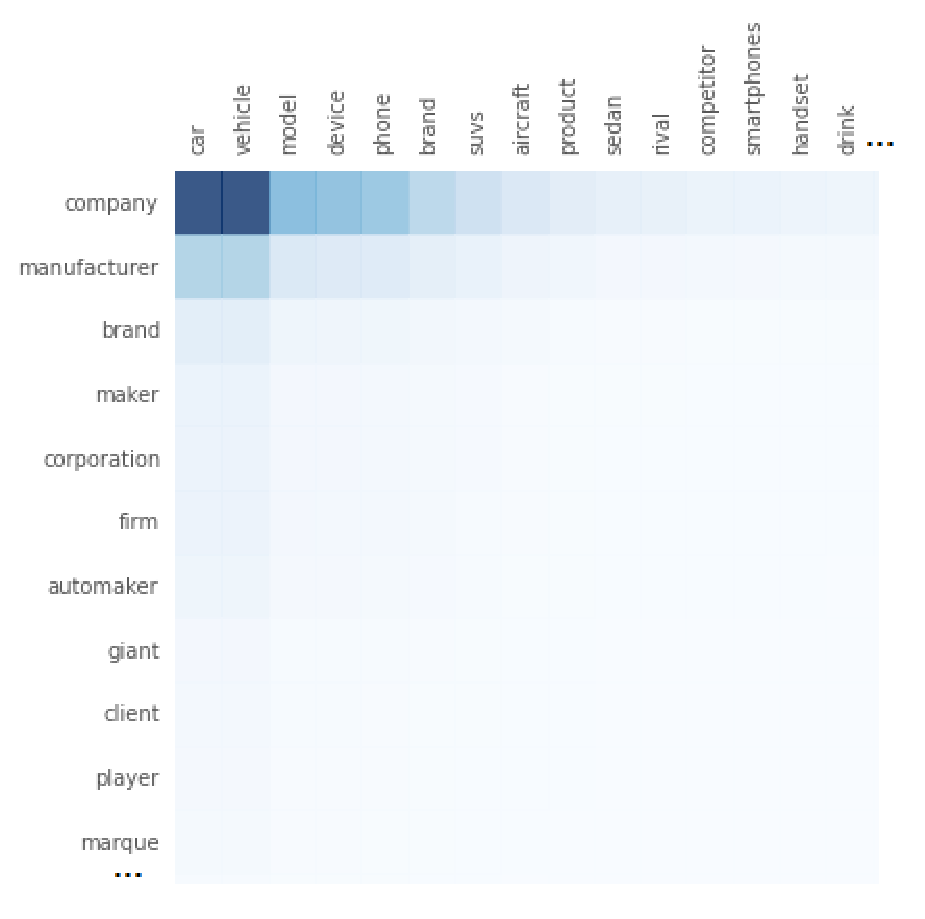
\epsfig{file=resources/ev_plot_manufacturer.eps,width=2.5in}
%\caption{$(c_1,c_2$) plot for attribute \term{Manufacturer}. } \label{fig:evplot}
%\end{figure}
%
%\begin{example}[Sense Disambiguation]
%Consider the following $(e1,a,e2)$ tuple \term{(iphone, manufacturer, apple)}. Suppose it is our query, where \term{apple}'s sense can either be a kind of \term{fruit} or a \term{company}.
%Fig.~\ref{fig:evplot} is a heatmap for all the concepts pairs $(c_1,c_2)$ of attributes \term{manufacturer}. The horizontal axis represents the $e_1$ and the vertical axis stands for $e_2$. The darker the blue is, the higher typicality it will be. In Fig.~\ref{fig:evplot}, We can observe that the top concepts of $e_2$ in the heatmap are \term{company, manufacturer,...} and top 10 pairs also does not include \term{fruit}. The intuition for this is that there exists thousands of $(e1,a,e2)$ tuple such as \term{(BMW\_Z4,manufacturer,BMW),(PlayStation\_4,manufacturer,Sony)} other than \term{(iphone, manufacturer, apple)} tuple, which results in a reasonable distribution.
%\label{exa:sd}
%\end{example}
%
%We further present a comparison of Eq.~\ref{eq:target_expand2_jr} and Eq.~\ref{eq:target_expand2_naive}, where the conceptualization is done with and without multiplying $\alpha(c_1,c_2)$.
%
%\begin{figure}[!htb]
%\centering
%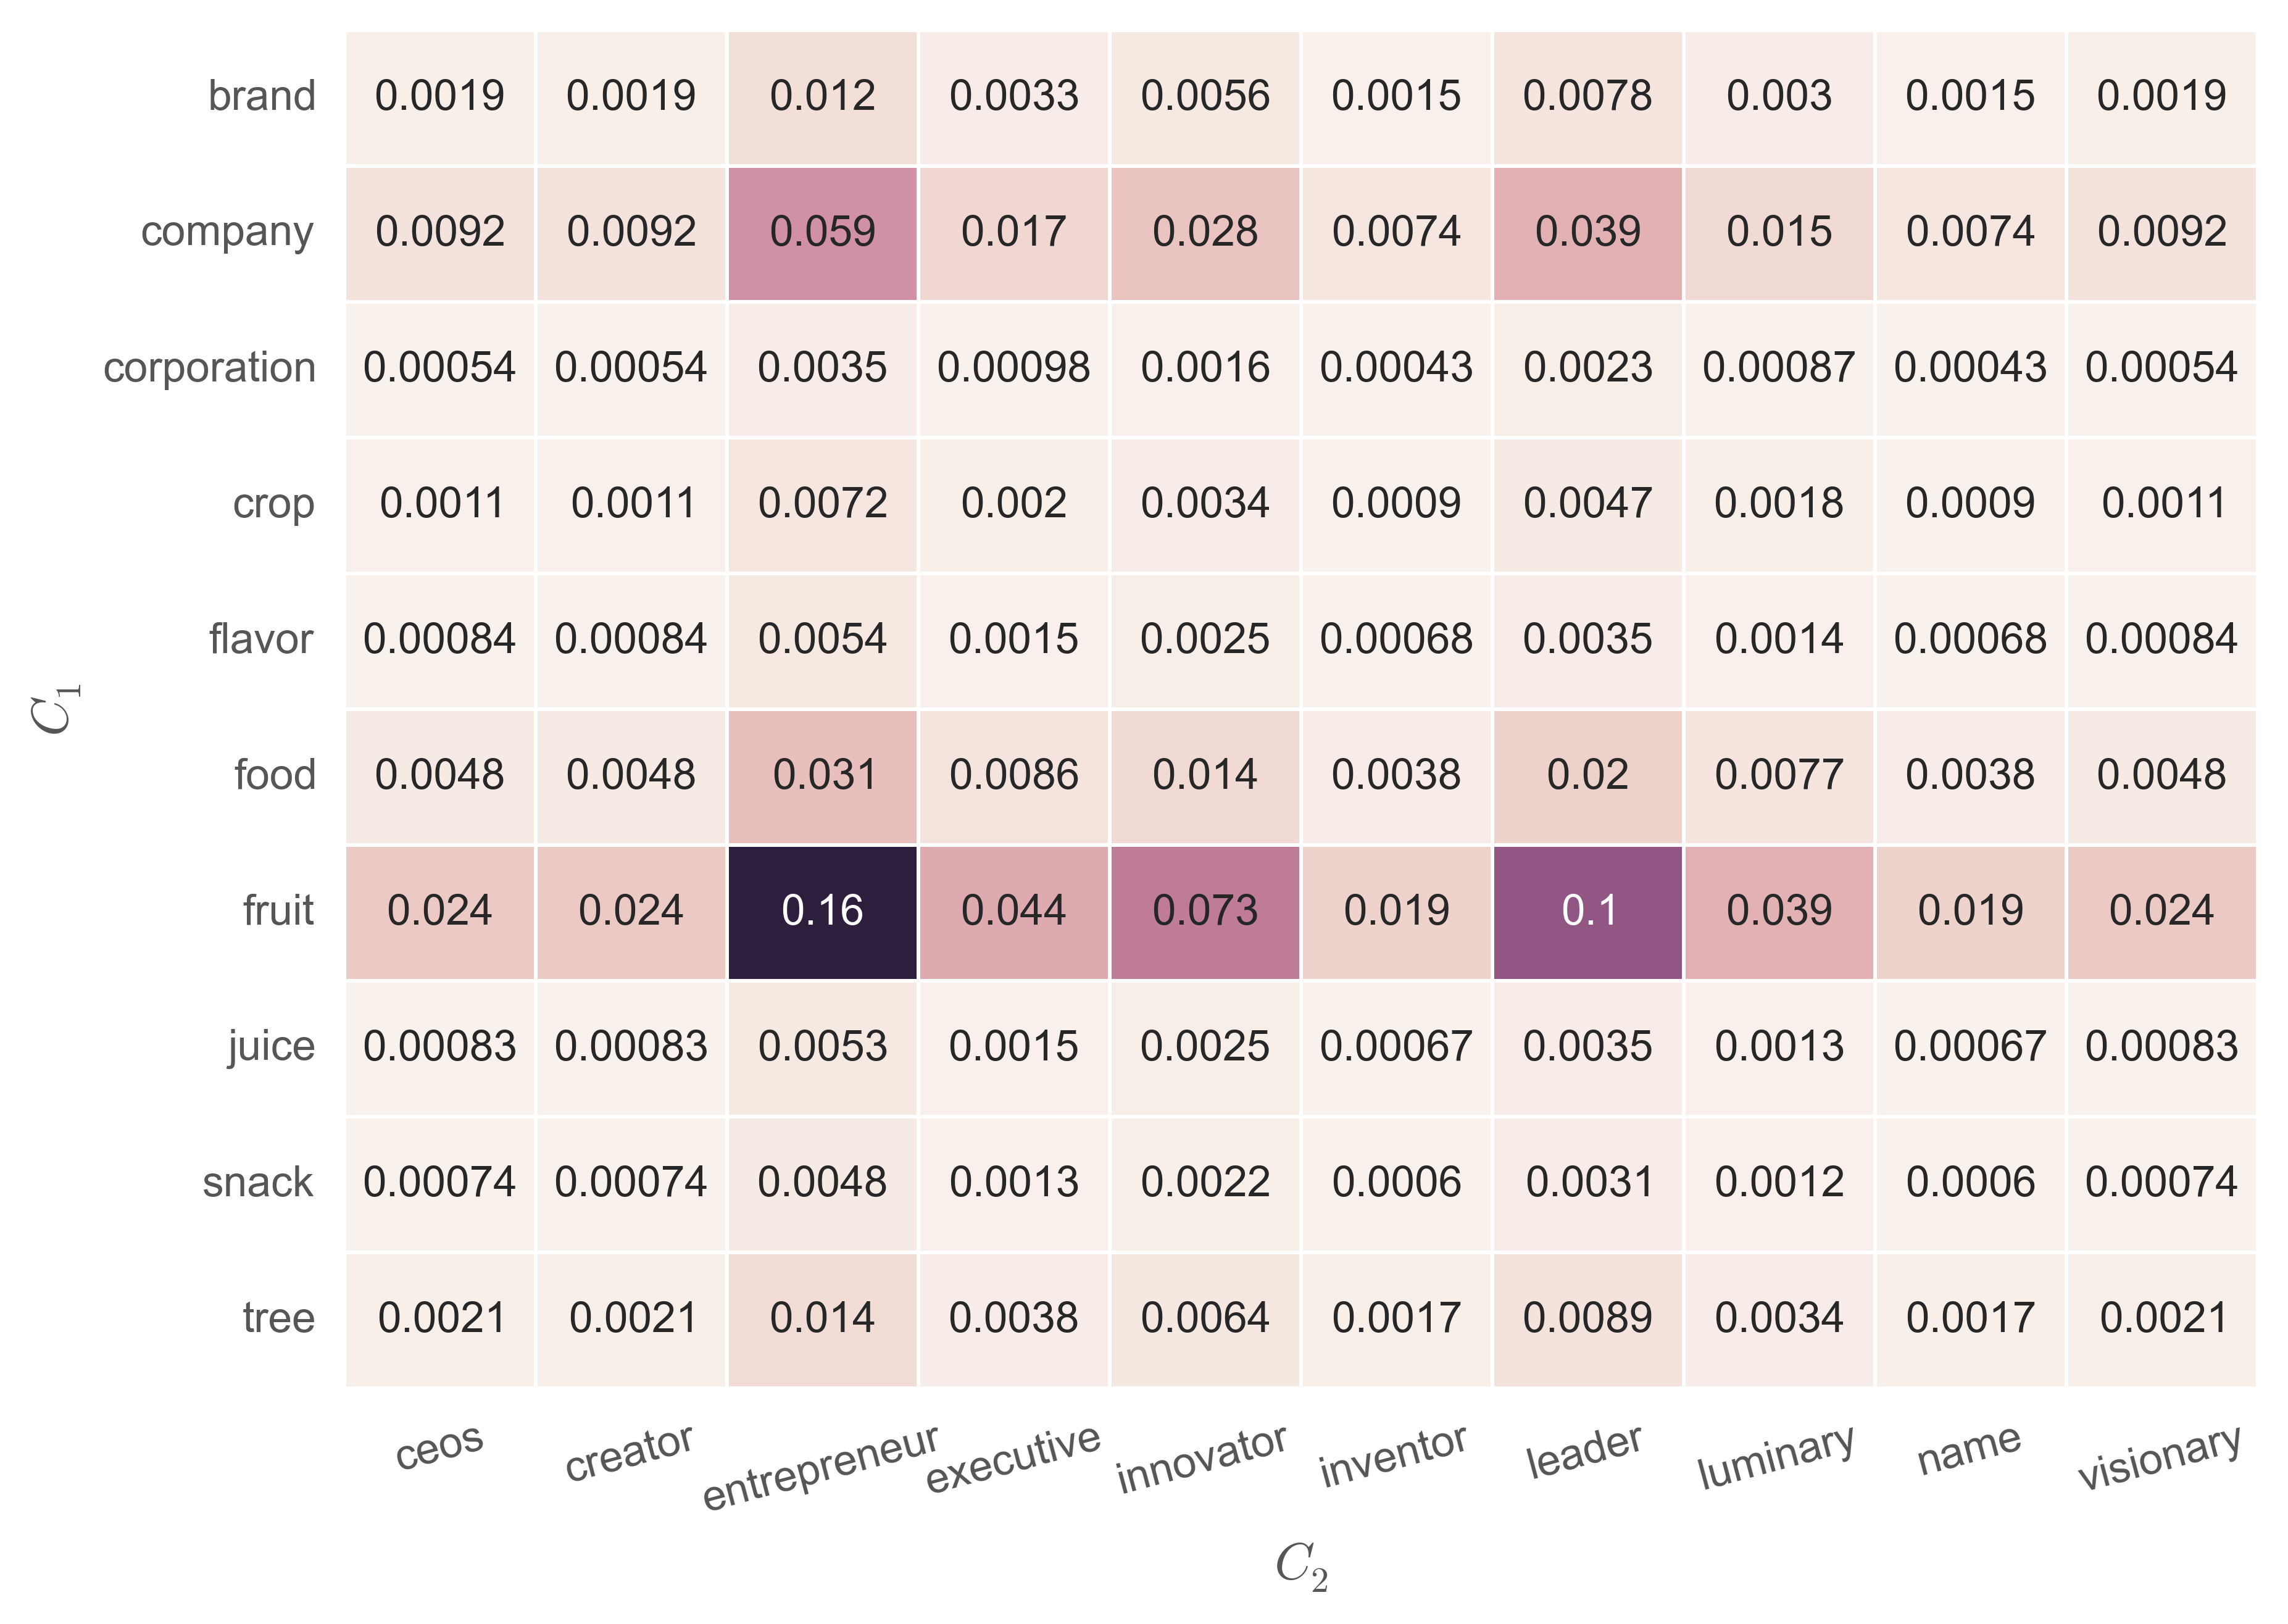
\epsfig{file=resources/df_for_plot_foundedBy.eps,width=\columnwidth }
%\caption{Distribution of $P(\langle c_1,c_2 \rangle|\langle e_1,e_2 \rangle )$ of attribute \at{foundedBy} \textbf{without} $\alpha$. }
%\label{fig:c1c2}
%\end{figure}
%
%\begin{figure}[!htb]
%\centering
%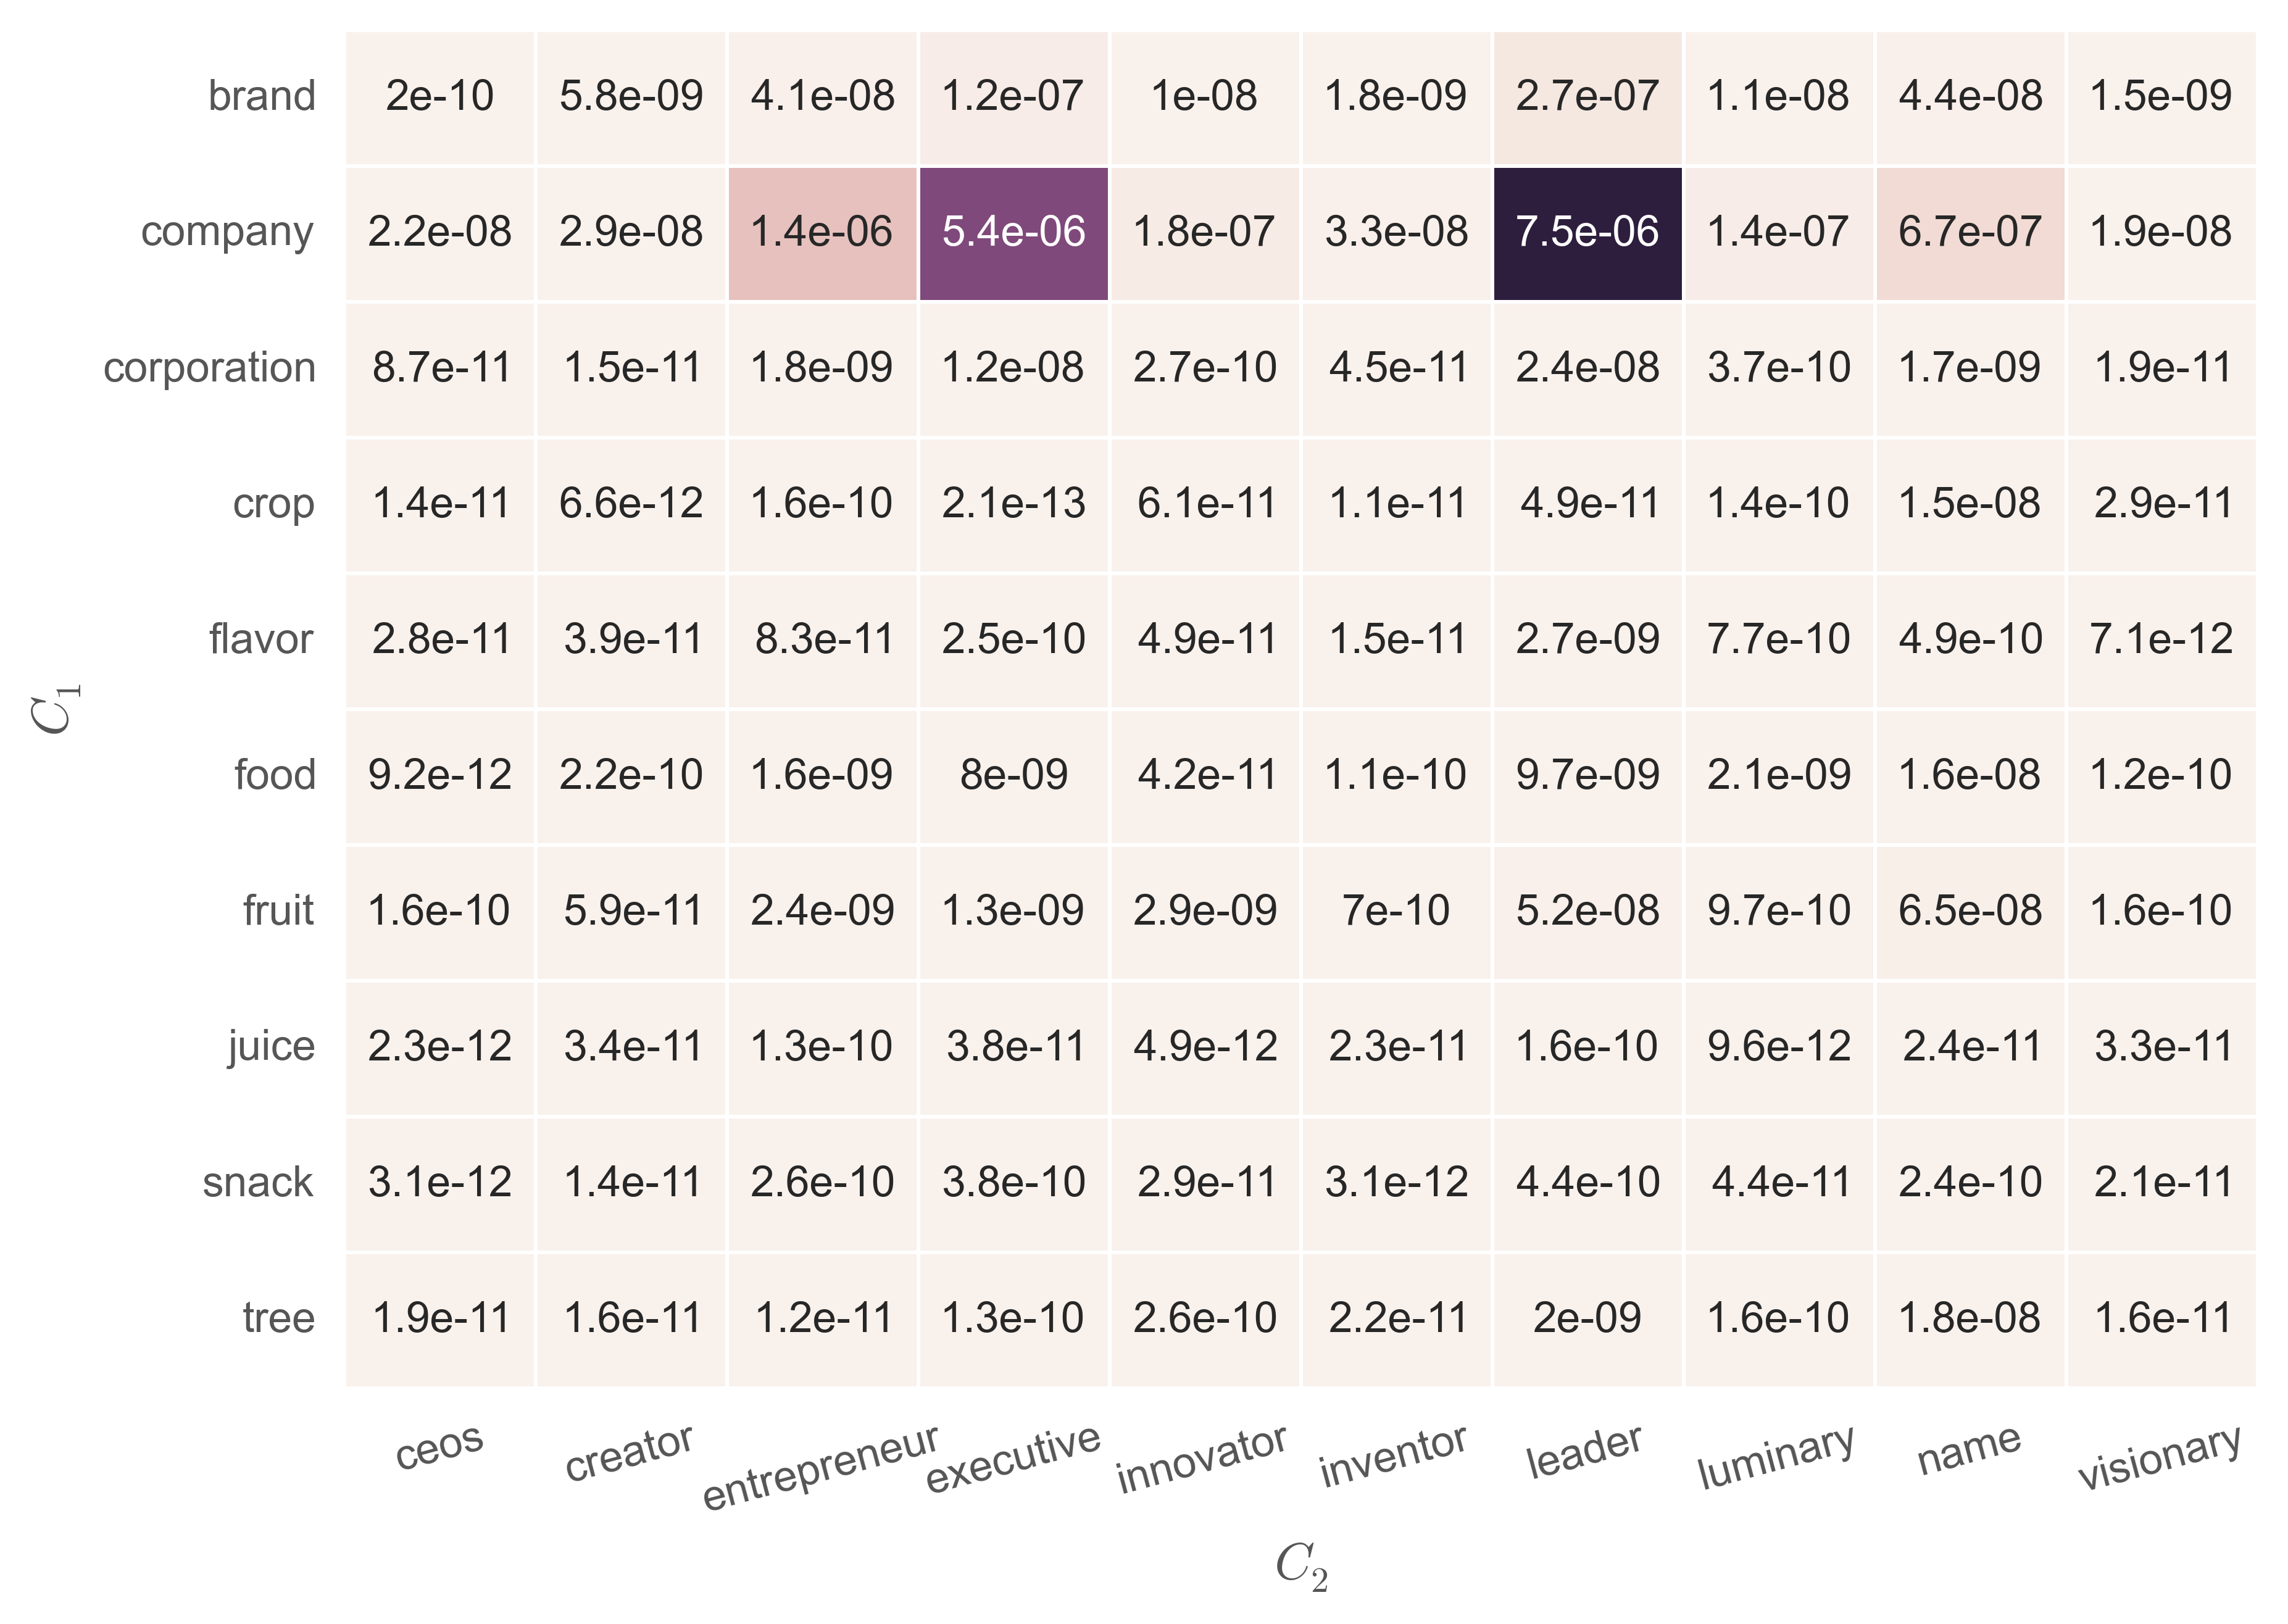
\epsfig{file=resources/df_for_plot_foundedBy_with_alpha_c1c2.eps,width=\columnwidth}
%\caption{Distribution of $P(\langle c_1,c_2 \rangle|\langle e_1,e_2 \rangle )$ of attribute \at{foundedBy} \textbf{with} $\alpha=P(\langle c_1,c_2 \rangle)$. }
%\label{fig:c1c2_alpha}
%\end{figure}
%
%\begin{figure}[!htb]
%\centering
%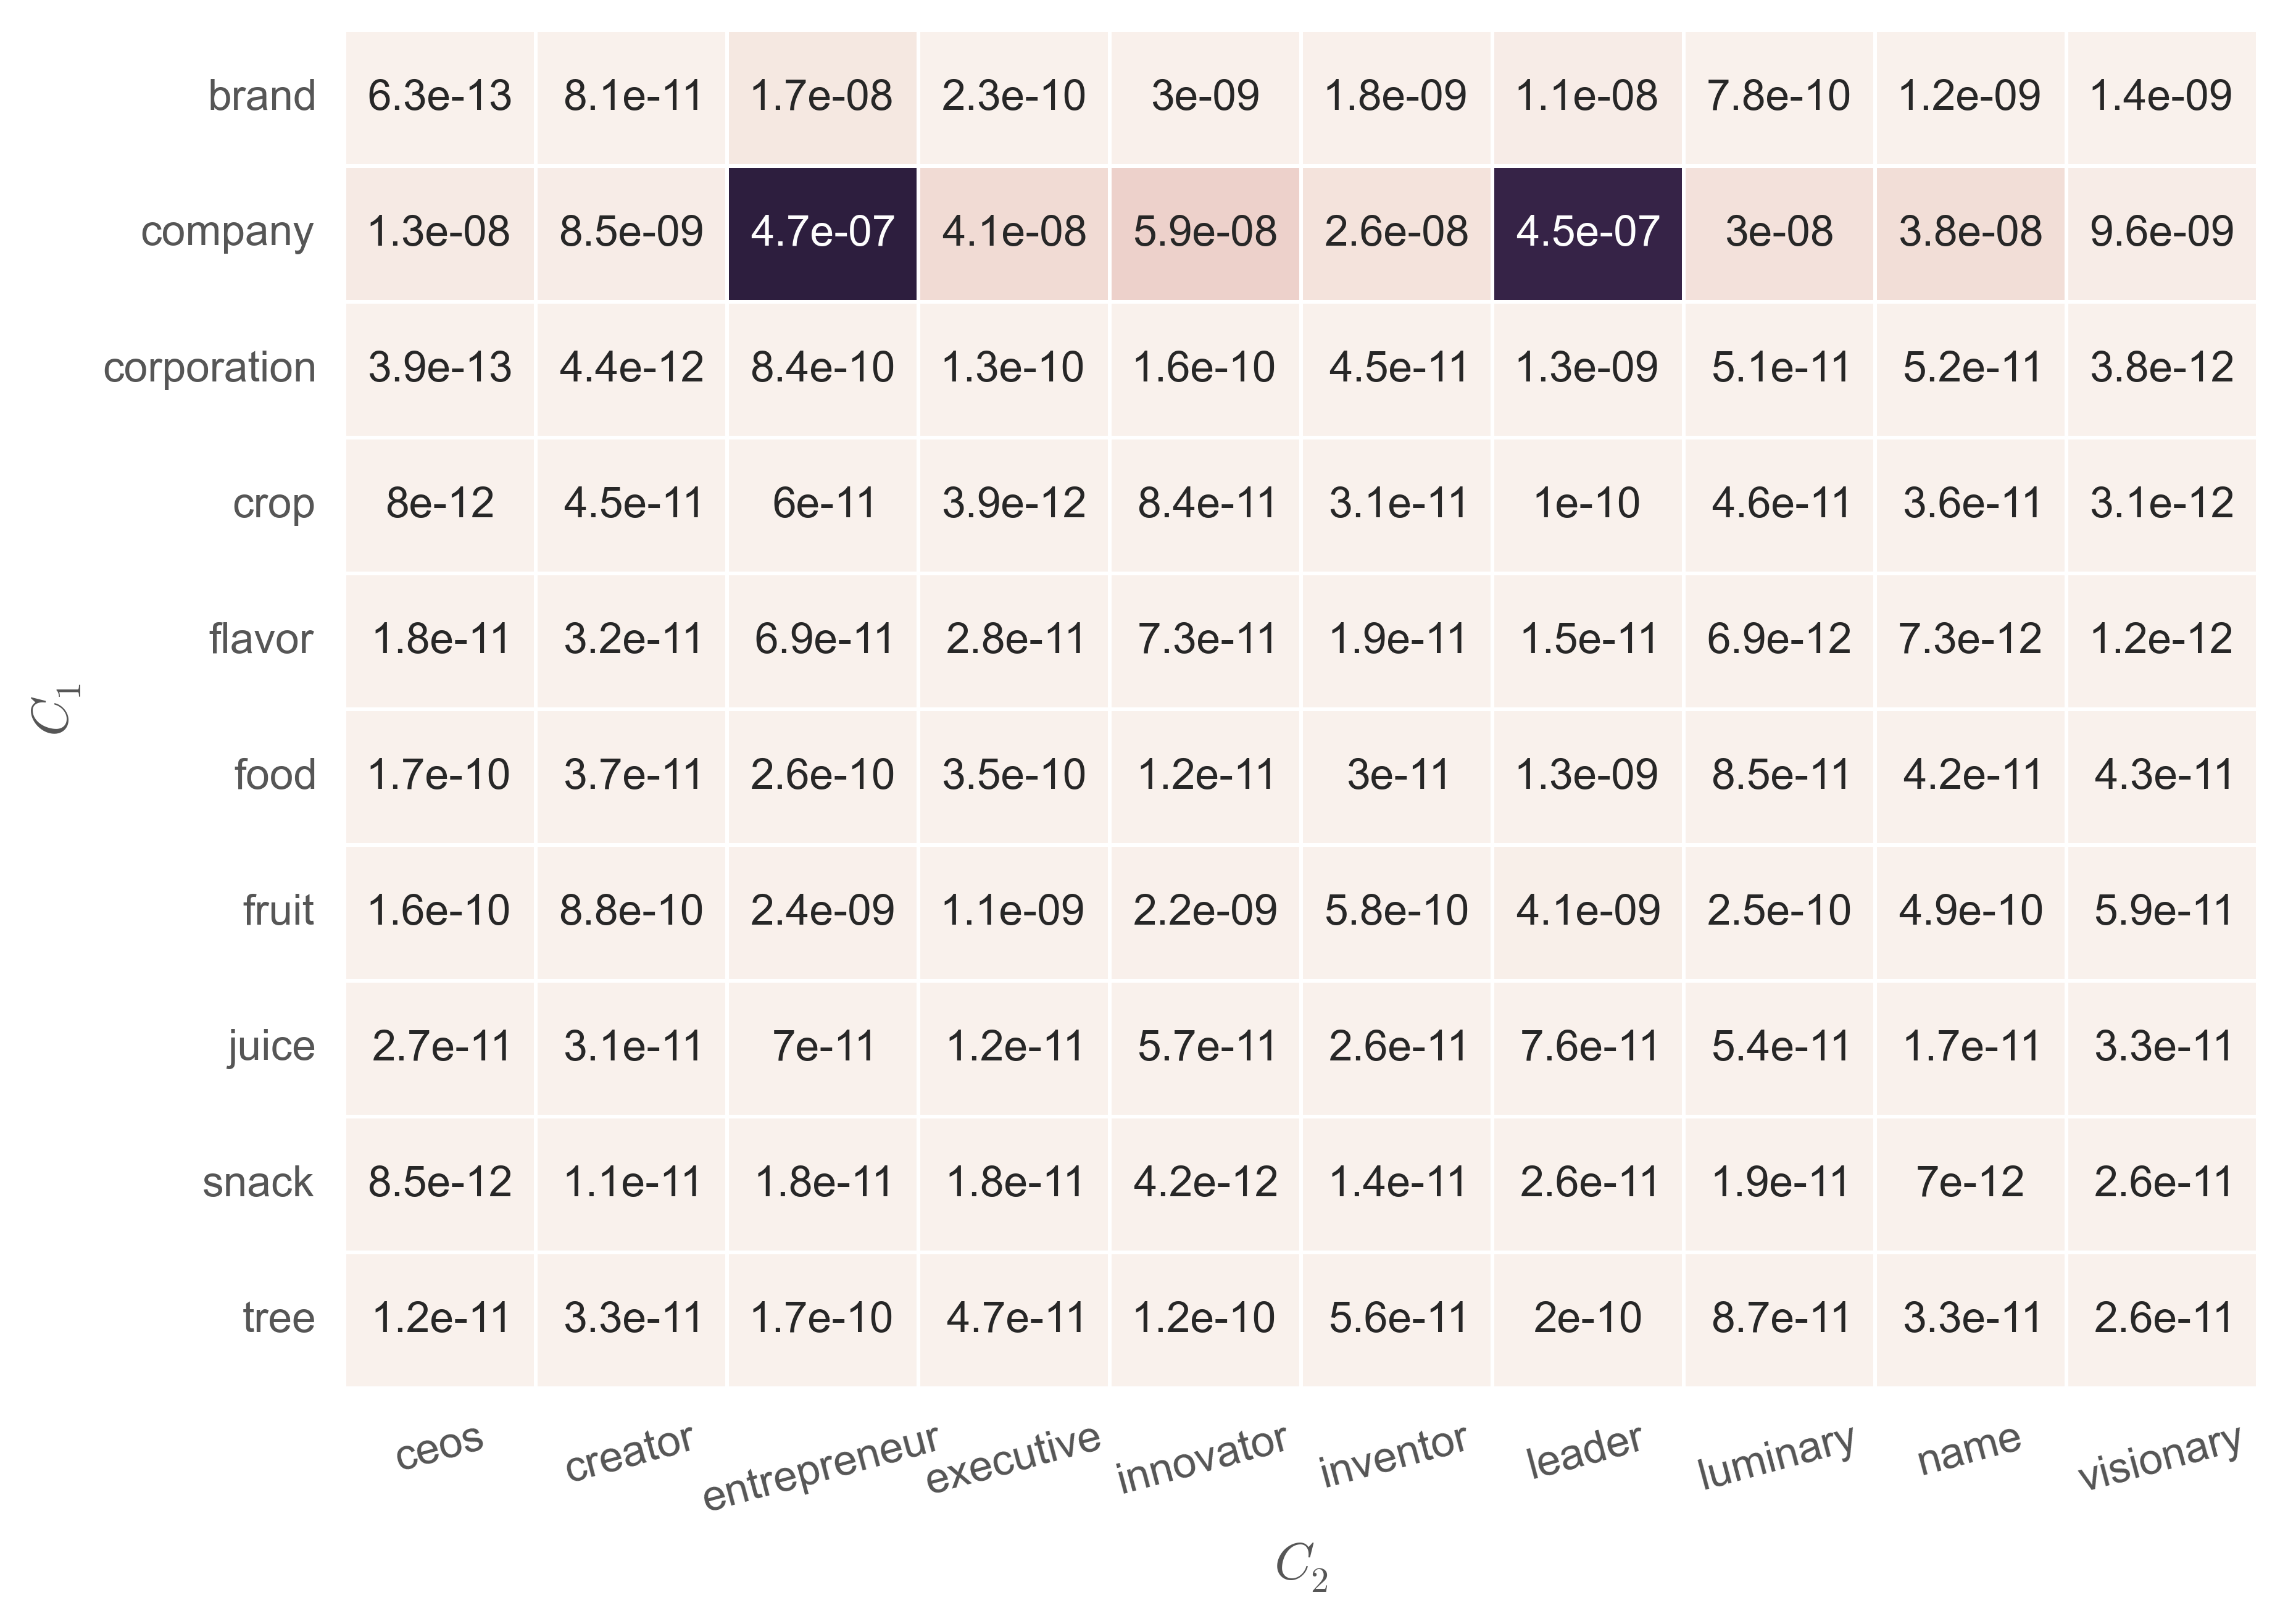
\epsfig{file=resources/df_for_plot_foundedBy_with_alpha.eps,width=\columnwidth}
%\caption{Distribution of $P(\langle c_1,c_2 \rangle|\langle e_1,e_2 \rangle )$ of attribute \at{foundedBy} \textbf{with} $\alpha=P(\langle c_1,c_2 \rangle|a)$. }
%\label{fig:c1c2_alpha_given_a}
%\end{figure}
%
%
%We present the visualization of the distribution of $P(\langle c_1,c_2 \rangle|\langle e_1,e_2 \rangle )$ for Eq.~\ref{eq:naive} in Figure~\ref{fig:c1c2} and for Eq.~\ref{eq:target_expand2_jr} in Figure~\ref{fig:c1c2_alpha}.
%The floats inside each box represents $P(\langle c_1,c_2 \rangle|\langle e_1,e_2 \rangle )$, when the pair $\langle c_1,c_2 \rangle$ does not exist, we add a small value to $\alpha$ and then do normalization for smoothing purpose.
\begin{figure}[!b]
%\vspace{-2mm}
\centering
\footnotesize
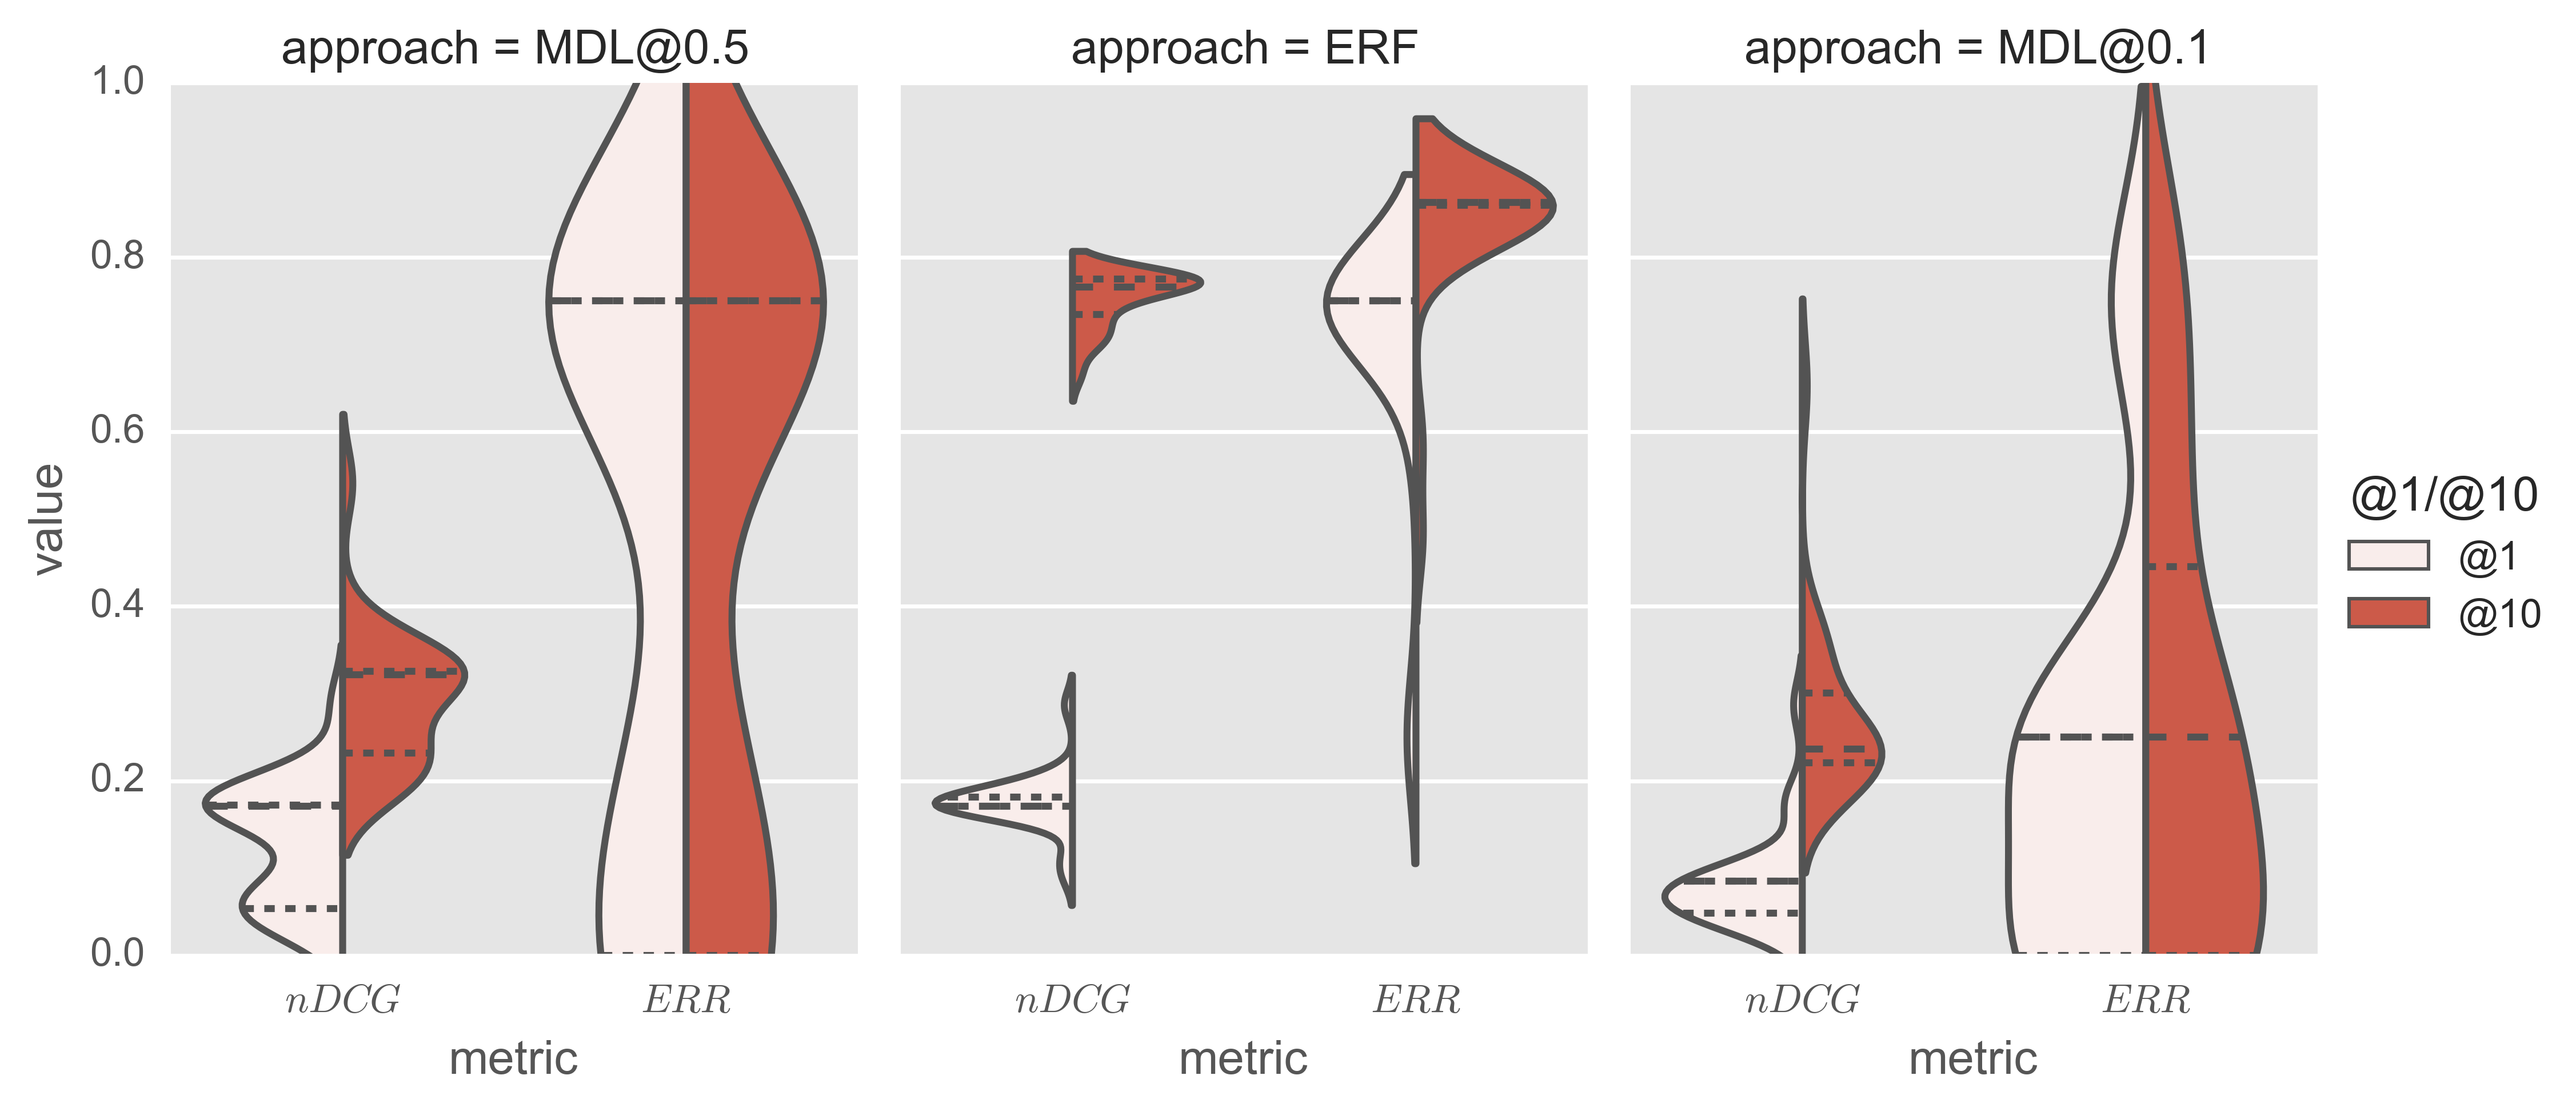
\epsfig{file=resources/violin_eval.eps,width=1.1\columnwidth}
\vspace{-8mm}
\caption{\small Distribution of human evaluation result for $P(\langle c_1,c_2 \rangle|a)$. \footnotesize The white part is metric@1 and the red part is metric@10. Dashed line means quartiles of the distribution. The $ERF$ in the middle is our result, compared with $MDL@\alpha=0.5$ (left) and $MDL@\alpha=0.1$(right). }
\label{fig:eva_violin_pc1c2ga}
\vspace{-4mm}
\end{figure}

%
%\begin{figure*}[htb]
%\centering
%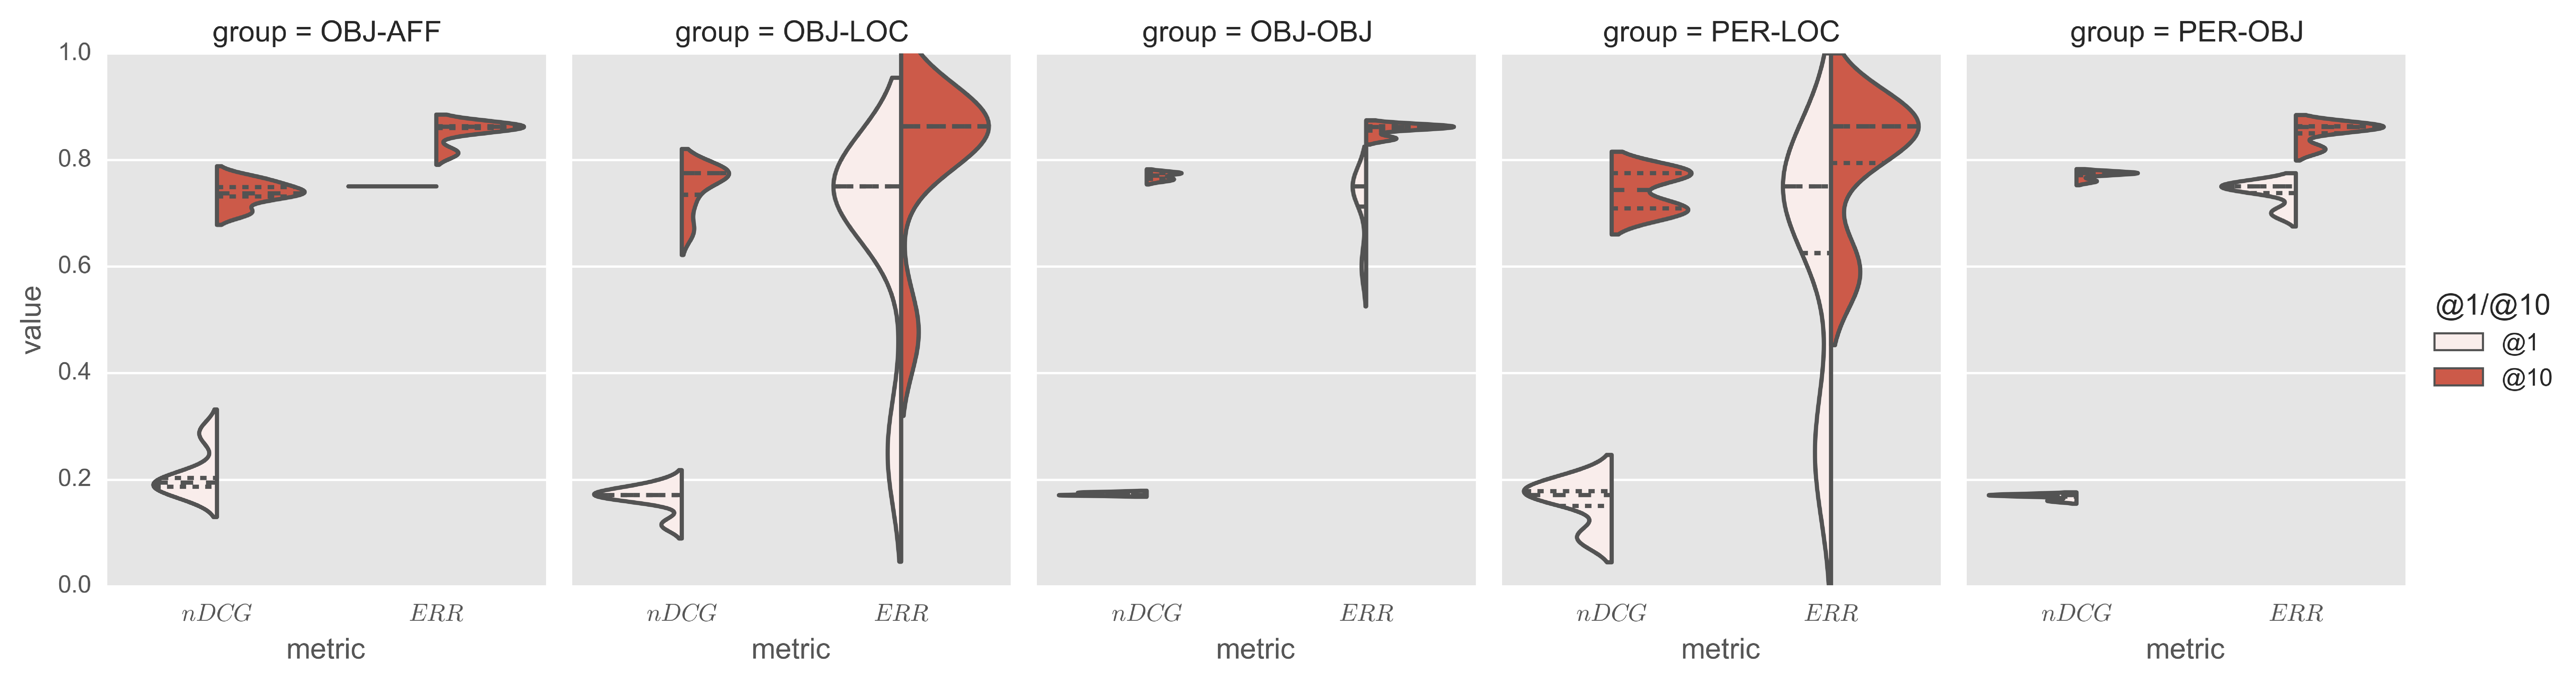
\epsfig{file=resources/violin_eval_group.eps,width=2.2\columnwidth}
%\vspace{-8mm}
%\caption{Distribution of human evaluation result for $P(\langle c_1,c_2 \rangle|a)$ produced by $ERF$. \small Each seperate graph represents a certain relation group.}
%\label{fig:eva_violin_group}
%\vspace{-6mm}
%\end{figure*}
%

\vspace{-4mm}
\paragraph*{Exp 4: Collective Conceptualization}
We compare our approach with an $MDL$ based collective conceptualization solution~\cite{sunconceptual}, which aims at generating a minimum set of conceptual labels that best summarize a bag of words.
In our case, the bag of words is replaced by a set of entities.
$MDL$ uses $\alpha$ to tune the balance between \ac{Minimality} and \ac{Coverage}. 
Bigger $\alpha$ lead to better coverage as well as general concepts.
We set the parameter $\alpha$ in $MDL$ to 0.5 for normal comparison and 0.1 for gaining more concept pairs.

In the experiment, we select 50 attributes from different relation groups (such as \at{PERSON-ORGNIZATION, PERSON-AFFLIATION,} etc.\ ) and manually evaluate the top 20 concept pairs for each attribute.
Volunteers give a score \textbf{2} for excellent concept pairs (e.g. \at{<company, entrepreneur>} for \at{FoundedBy}), \textbf{1} for correct while not appropriate ones (e.g. \at{<song, celebrity>} for \at{writer} ), and \textbf{0} for wrong concept pairs (e.g. \at{<topic, Country>} for \at{SpokenIn}).
We present the human evaluated score in Figure~\ref{fig:eva_violin_pc1c2ga}.
We also show the evaluation results on each relation relation group produced by $ERF$ in Figure~\ref{fig:eva_violin_group}.

\begin{table}[!hb]
  \vspace{-4mm}
  \centering
  \small
  \caption{Joint Conceptualization with and without $\alpha$}
    \begin{tabular}{rrrr}
    \toprule
    $e_1$                               & $e_2$                               & $c_1 $  without $\alpha$       & $c_1$  with $\alpha$ \\
    \midrule
    columbia                            & barack obama                        & country                    & \textbf{school }\\
    apple                               & steve jobs                          & fruit                & \textbf{company} \\
   da vinci code           & ron howard                       & book                     & \textbf{film} \\
    spa                                 & belgium                             & facility                  & \textbf{place} \\
    \bottomrule
    \end{tabular}%
  \label{tab:expjc}%
  \vspace{-2mm}
\end{table}%


From the results we can see that $ERF$ always produces the best result in terms of $nDCG@1$ and $nDCG@10$.
We can observe a significant increase in the $nDCG@10$ score for $ERF$ while not much increase in $MDL$-based approach. Because $MDL$ tends to give as few concepts as possible and sacrifices the coverage when $\alpha$ is small. The $nDCG@1$ score is reasonably low since usually there are more than one pair of correct concepts.

$ERR@1$ and $ERR@10$ measure vary not that much due to its user-behavioral instinct. In general, a real user pays less attention to the lower-ranked pairs after he/she find the correct concept pair.
The results show that 
 $ERF$ always performs best and gains an slight increase in $ERR@10$ compared to $ERR@1$.
 The results are consistent across different groups of relationships.



\vspace{-4mm}
\paragraph*{Case Study}
We show some of the relations that has been retrieved by our method in Table~\ref{tab:results}.
\nop{The first 2 columns show the query entity pair.
The 3rd column is the relation retrieved by $ERF$ with a confidence score in the 4th column.
Note that we combine the relationships of $\langle e_1,e_2\rangle$ and $\langle e_2,e_1\rangle$ together.
For example the relation \at{commander} of \at{<adolf hitler,world war ii>} is actually the attribute of \at{<world war ii, adolf hilter>}. }From the table, we can see that most top one relation is the right attribute between the entity pair.
For some entity pairs, the top 2 or 3 relations are also reasonable, for example the \at{<apple, steve jobs>} case.
All these case studies sufficiently show the effectiveness of $ERF$.
% Table generated by Excel2LaTeX from sheet 'Sheet1'
\begin{table}[!t]
%\vspace{6mm}
  \centering
  \caption{Top Three Results Produced by $ERF$}
  \small
    \begin{tabular}{cccr}
    \toprule
    Entity1 & Entity2 & Relation & Score ($\times10^{-3}$) \\
    \midrule
%    \multicolumn{1}{c}{\multirow{3}{*}{\parbox{1cm}{\small Sherlock Holmes}}} & \multicolumn{1}{c}{\multirow{3}[0]{*}{united kingdom}} & anthem & 7.0 \\
%    \multicolumn{1}{c}{} & \multicolumn{1}{c}{} & firstAppearance & 4.5 \\
%    \multicolumn{1}{c}{} & \multicolumn{1}{c}{} & allegiance & 4.4 \\
%    \hline
    \multicolumn{1}{c}{\multirow{3}{*}{\parbox{1cm}{\centering apple}}} & \multicolumn{1}{c}{\multirow{3}[0]{*}{steve jobs}} & foundedBy & 15.4 \\
    \multicolumn{1}{c}{} & \multicolumn{1}{c}{} & keyPerson & 9.9 \\
    \multicolumn{1}{c}{} & \multicolumn{1}{c}{} & successor & 8.1 \\
    \hline
    \multicolumn{1}{c}{\multirow{3}{*}{\parbox{1cm}{\centering\small\vspace{-1.6mm}  Adolf Hitler}}} & \multicolumn{1}{c}{\multirow{3}[0]{*}{world war ii}} & commander & 37.7 \\
    \multicolumn{1}{c}{} & \multicolumn{1}{c}{} & battle & 22.1 \\
    \multicolumn{1}{c}{} & \multicolumn{1}{c}{} & ceo   & 0.024 \\
    \hline
    \multicolumn{1}{c}{\multirow{3}{*}{\parbox{1cm}{\centering Microsoft}}} & \multicolumn{1}{c}{\multirow{3}[0]{*}{redmond}} & locationCity & 82.5 \\
    \multicolumn{1}{c}{} & \multicolumn{1}{c}{} & foundationPlace & 47.1 \\
    \multicolumn{1}{c}{} & \multicolumn{1}{c}{} & location & 36.9 \\
    \hline
    \multicolumn{1}{c}{\multirow{3}{*}{Titanic}} & \multicolumn{1}{c}{\multirow{3}[0]{*}{James Cameron}} & director & 124.4 \\
    \multicolumn{1}{c}{} & \multicolumn{1}{c}{} & cinematography & 96.4 \\
    \multicolumn{1}{c}{} & \multicolumn{1}{c}{} & editing & 80.1 \\
    \hline
    \multicolumn{1}{c}{\multirow{3}{*}{Titanic}} & \multicolumn{1}{c}{\multirow{3}[0]{*}{Leonardo Dicaprio}} & starring & 49.6 \\
    \multicolumn{1}{c}{} & \multicolumn{1}{c}{} & narrator & 37.2 \\
    \multicolumn{1}{c}{} & \multicolumn{1}{c}{} & producer & 13.0 \\
    \hline
    \multicolumn{1}{c}{\multirow{3}{*}{\parbox{1cm}{\centering \vspace{-1mm} Harry Potter}}} & \multicolumn{1}{c}{\multirow{3}[0]{*}{J K rowling}} & notableWork & 16.9 \\
    \multicolumn{1}{c}{} & \multicolumn{1}{c}{} & author & 15.5 \\
    \multicolumn{1}{c}{} & \multicolumn{1}{c}{} & coverArtist & 14.9 \\
    \bottomrule
    \end{tabular}%
  \label{tab:results}%
\vspace{-8mm}
\end{table}%


%\subsection{Selectional Preference}
